\documentclass[11pt,a4paper]{article}

\usepackage[margin=0.9in]{geometry}
\usepackage{graphicx}
\usepackage{booktabs}
\usepackage{float}
\usepackage{natbib}
\usepackage{newtxtext,newtxmath}
\usepackage[hidelinks]{hyperref}

\graphicspath{{./}}
\emergencystretch=2em

\title{Thieulot spherical Stokes benchmark}
\author{}
\date{}

\begin{document}

\maketitle
\vspace{-2.0em}

\section{Benchmark description}

The spherical Stokes benchmark of \citet{thieulot2017} provides a closed-form solution for incompressible viscous flow in a spherical shell. The velocity is tangential on both spherical boundaries, the viscosity varies radially according to a power law, and analytical expressions are available for the density, velocity, pressure, body force, and full stress tensor. The problem therefore provides a stringent three-dimensional verification test for curved-domain Stokes discretisations and for post-processing quantities derived from the stress field.

We consider the two cases used in the original benchmark: \(m=-1\), for which the viscosity is constant, and \(m=3\), for which the viscosity changes by a factor of 16 across the shell. The Underworld3 calculations use a \(P_2P_1\) Taylor--Hood element pair, with quadratic velocity and linear pressure. Mesh resolution is reported using the nominal cell size \(h=1/8,\ldots,1/128\). Velocity and pressure errors are evaluated using relative volume \(L_2\) norms, while radial normal-stress errors are evaluated using relative boundary \(L_2\) norms on the inner and outer spherical surfaces.

\begin{figure}[H]
    \centering
    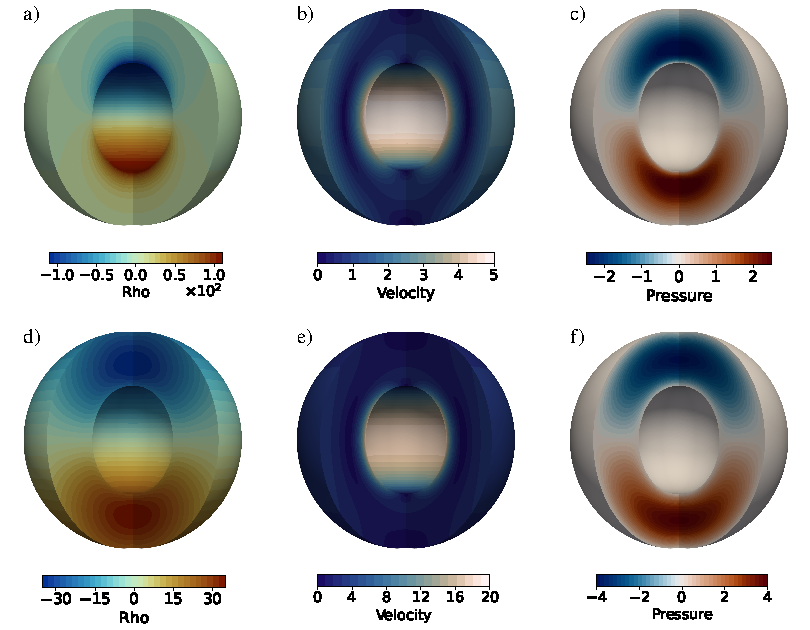
\includegraphics[width=0.92\linewidth]{figure_2_thieulot_analytical.pdf}
    \caption{Analytical density, velocity magnitude, and pressure fields for the Thieulot spherical benchmark. The upper row shows the \(m=-1\) case and the lower row shows the \(m=3\) case.}
    \label{fig:thieulot_analytical_fields}
\end{figure}

Figure~\ref{fig:thieulot_analytical_fields} shows the analytical density, velocity magnitude, and pressure fields. Both cases satisfy the no-normal-flow condition on the inner and outer boundaries while retaining non-zero tangential velocity. The \(m=3\) case uses the same geometry but introduces a stronger radial viscosity variation, and therefore provides a more demanding test of the pressure and stress recovery than the constant-viscosity case.

\section{Velocity and pressure convergence}

\begin{figure}[H]
    \centering
    
\includegraphics[width=0.98\linewidth]{figures_4_5_thieulot_convergence.pdf}
    \caption{Convergence of the volume \(L_2\)-norm velocity and pressure errors for the \(P_2P_1\) discretisation.}
    \label{fig:thieulot_velocity_pressure_convergence}
\end{figure}

\begin{table}[H]
    \centering
    
\includegraphics[width=0.98\linewidth]{table_figures_4_5_convergence.pdf}
    \caption{Velocity and pressure \(L_2\)-norm errors and observed convergence rates for \(m=-1\) and \(m=3\).}
    \label{tab:thieulot_velocity_pressure_rates}
\end{table}

The measured convergence is consistent with the expected behaviour of Taylor--Hood elements for smooth Stokes solutions. For a \(P_2P_1\) discretisation, the expected minimum rates are third order for the velocity in the \(L_2\) norm and second order for the pressure in the \(L_2\) norm, provided the solution is sufficiently regular \citep[e.g.][]{girault1986,boffi2013}. These rates are also consistent with the spherical-shell results reported by \citet{thieulot2017} and with later analytical verification studies in curved shell geometries \citep{kramer2021,davies2022}. In the present calculations, the velocity error approaches \(O(h^3)\) for both \(m=-1\) and \(m=3\), while the pressure error approaches \(O(h^2)\) at the finest resolutions. The rates on the coarser meshes are less regular, particularly for pressure, reflecting pre-asymptotic behaviour and the larger error constants associated with curved geometry and radial viscosity variation.

\section{Boundary metric convergence}

\begin{figure}[H]
    \centering
    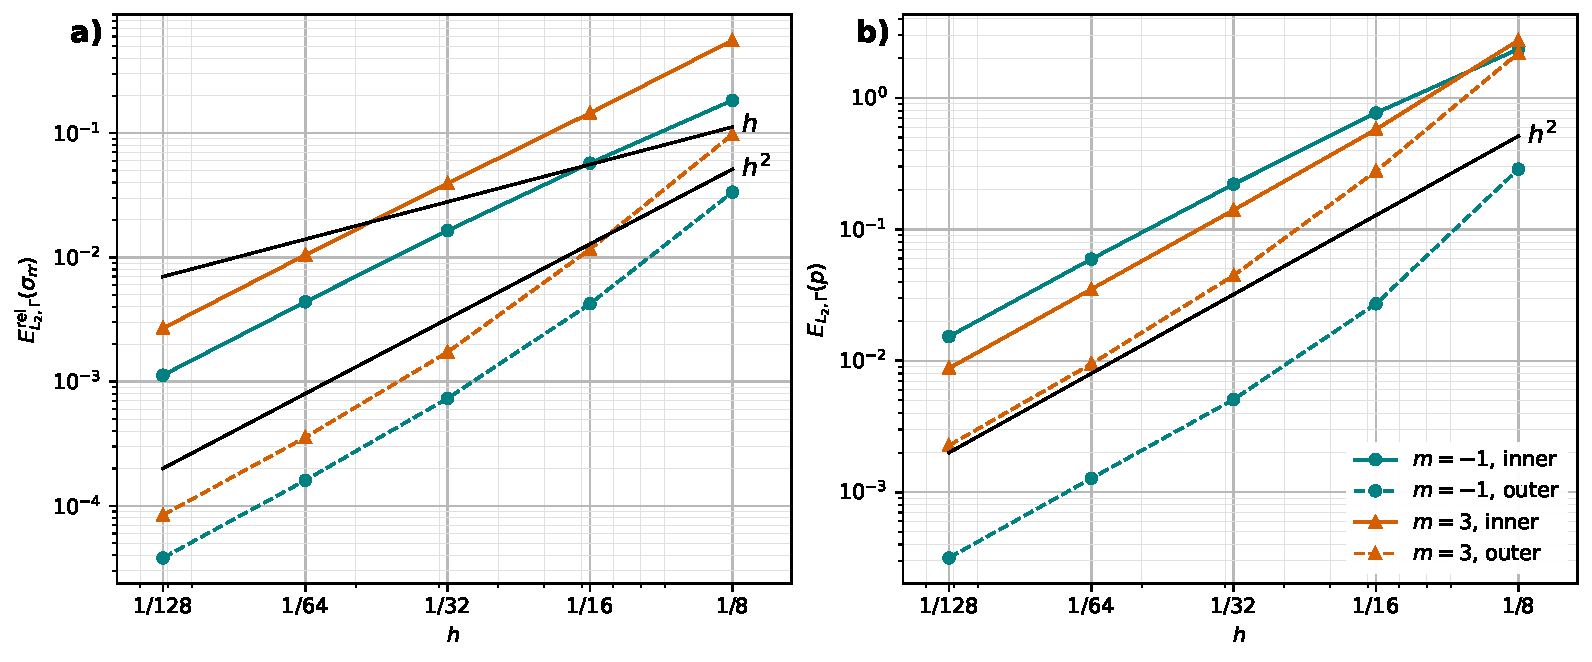
\includegraphics[width=0.98\linewidth]{boundary_metric_convergence.pdf}
    \caption{Convergence of boundary radial normal-stress and pressure errors. Solid lines denote the inner boundary and dashed lines denote the outer boundary.}
    \label{fig:thieulot_sigma_rr_convergence}
\end{figure}

\begin{table}[H]
    \centering
    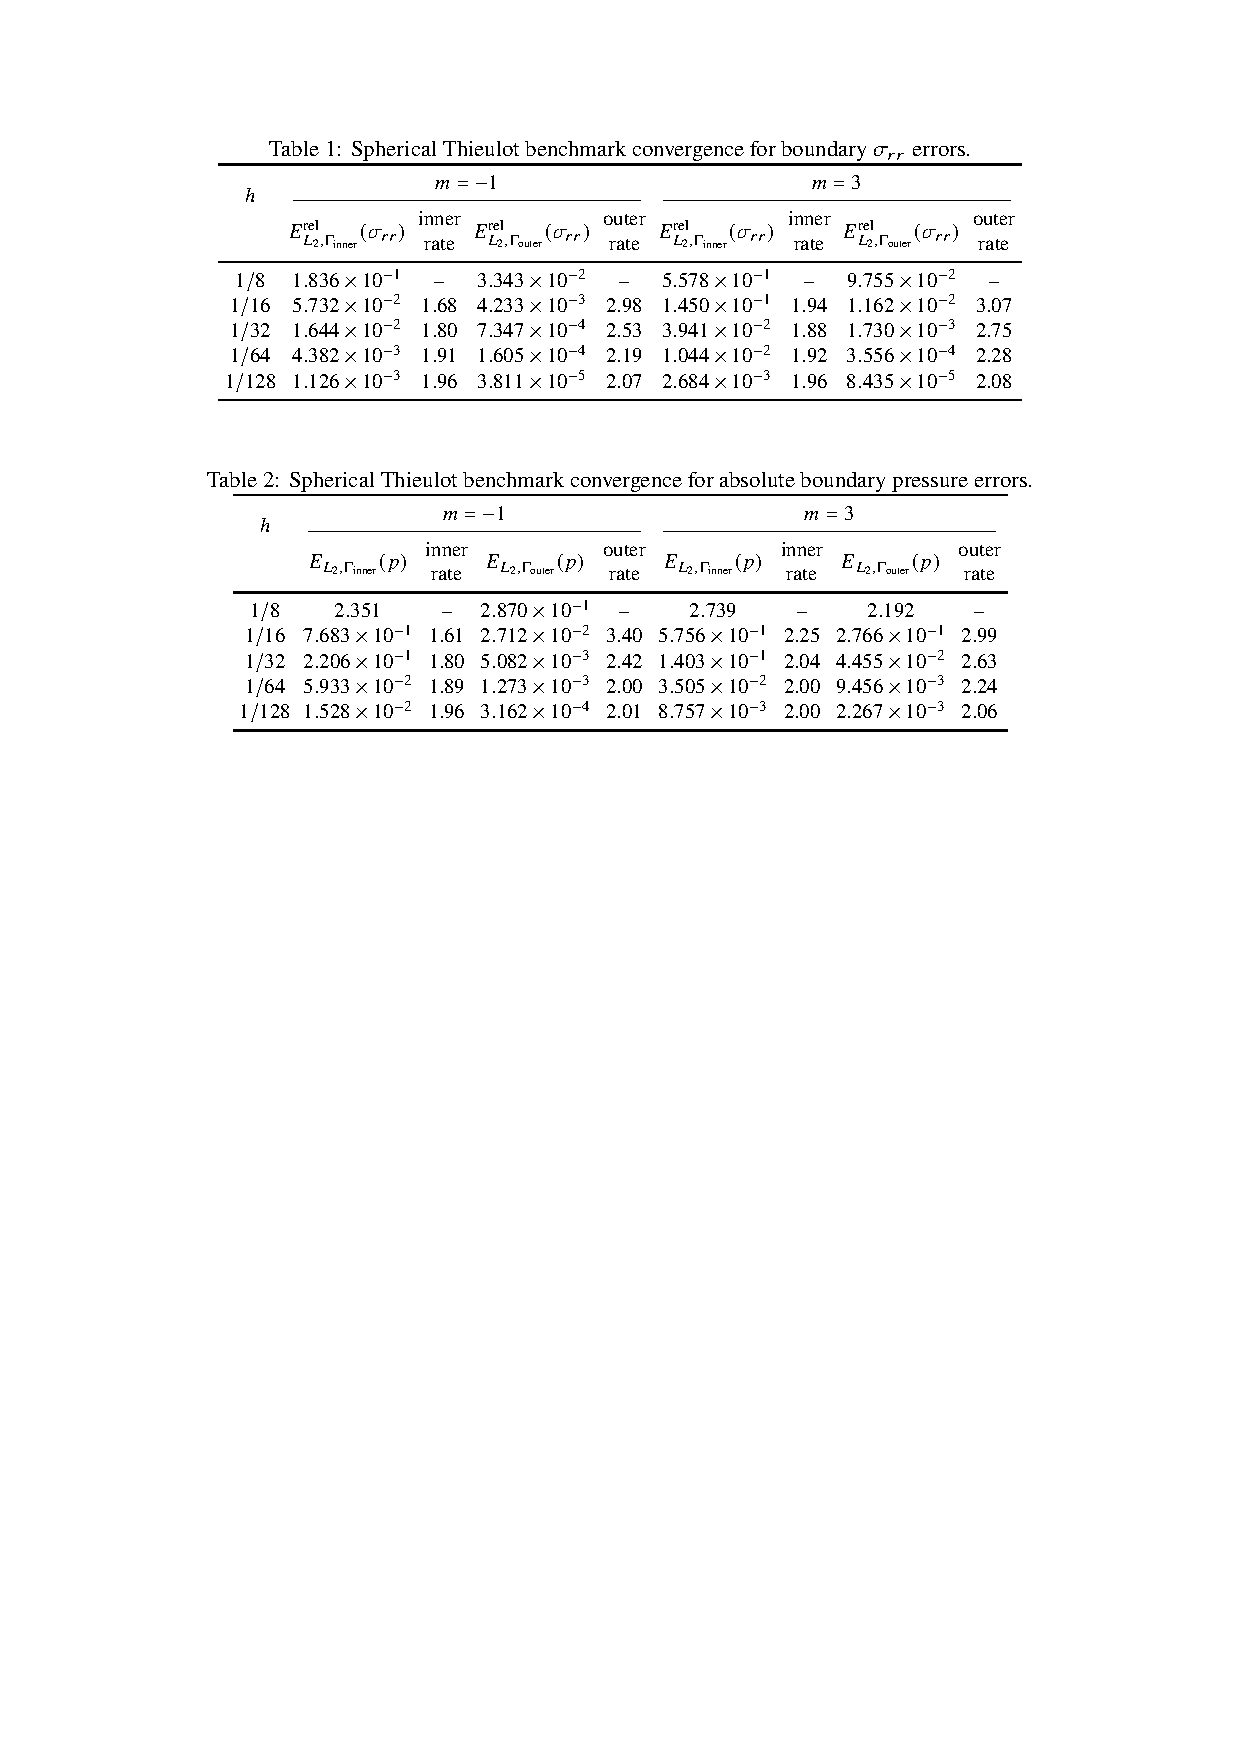
\includegraphics[width=0.98\linewidth]{table_boundary_metric_convergence.pdf}
    \caption{Boundary \(\sigma_{rr}\) and pressure \(L_2\)-norm errors with observed convergence rates for the inner and outer spherical surfaces.}
    \label{tab:thieulot_sigma_rr_rates}
\end{table}

Although \citet{thieulot2017} derive the full analytical stress tensor, the published benchmark reports convergence only for velocity and pressure. Here, the radial normal stress, \(\sigma_{rr}\), is included as an additional boundary diagnostic. This quantity is relevant for geodynamic Stokes solvers because surface normal stress enters dynamic-topography calculations and has been used in previous spherical-shell verification studies \citep{zhong1993,zhong2008,liu2019,kramer2021}. In related analytical spherical-shell tests, \citet{kramer2021} report second-order convergence for boundary normal stress. The Underworld3 results show the same asymptotic trend: the inner-boundary errors approach second-order convergence for both \(m=-1\) and \(m=3\), and the outer-boundary errors also approach \(O(h^2)\) at the finest resolutions.

The absolute magnitude of the inner- and outer-boundary stress errors differs even though the asymptotic rates are similar. This is expected. The convergence rate measures the exponent \(p\) in an error model \(E \approx C h^p\), whereas the prefactor \(C\) depends on the local analytical stress amplitude, the boundary surface area, quadrature, curvature, and the way pressure and recovered deviatoric-stress errors combine on each surface. Because the inner and outer boundaries have different radii and different analytical values of \(\sigma_{rr}\), and because the relative boundary norms are normalised independently on each surface, the two curves need not overlap. The relevant verification criterion is therefore the asymptotic slope, not equality of the error constants.

\section{Summary}

The Thieulot spherical benchmark verifies the Underworld3 Stokes discretisation in a curved three-dimensional shell for both constant and radially varying viscosity. The \(P_2P_1\) calculations recover the expected \(O(h^3)\) velocity convergence and \(O(h^2)\) pressure convergence for smooth analytical solutions. The radial normal-stress diagnostic also converges at approximately second order on both shell boundaries, consistent with related spherical-shell stress-verification studies. These results support the use of this benchmark as a production verification case for velocity, pressure, and boundary-stress post-processing in Underworld3.

\bibliographystyle{plainnat}
\bibliography{thieulot_spherical_benchmark_report_refs}

\end{document}
